\documentclass{article}
\usepackage[utf8]{inputenc}
\usepackage{biblatex}
\usepackage{graphicx}
\usepackage{float}
\usepackage[left=1in,top=1in,right=1in,bottom=1in,nohead]{geometry}
\usepackage{enumitem}
\usepackage[colorlinks]{hyperref}
\hypersetup{
    urlcolor=blue,
    }
\addbibresource{./citations.bib}


\newcommand{\fref}[2][]{%
  \ifthenelse{\equal{#1}{}}%
	{Fig.~\ref{fig:#2}}%
	{Figure~\ref{fig:#2}}}

%================================================================================
% main document
\title{Rubik's Cube Solver}
\author{HMC CS144 SciComp Final Project}
\date{Adam Walker, \t May 7, 2021}

\begin{document}
\maketitle

%========================================
\section{Introduction}

A Rubik's Cube is a 3D puzzle where performing moves changes the locations of various colored stickers. The original 3x3x3 puzzle consists of six faces, each with nine stickers arranged in a three by three grid. The object is to solve the puzzle such that all stickers on a given face are the same color. A variety of methods have been developed to solve a Rubik's Cube. Some methods are better for speedsolving, in which a human tries to solve the puzzle as quickly as possible \cite{speedcubing}. 

A Rubik's cube solver is a program that takes as input a configuration of stickers, and outputs a sequence of moves to solve the puzzle. Computer solvers have numerous implications for the speedsolving community. Solvers have been used in recent years to generate new algorithms (sequences of moves that affect a particular subset of stickers in a particular way) for speedsolvers. Counter intuitively, computerized solvers are also the backbone for generating scramble sequences. This is important for speedsolving competitions, which rely on scrambling programs to ensure that all competitors are given puzzles that are comparable in difficulty \cite{wca-scrambles}.

% Modern scrambling programs rely on generating a random scramble state (i.e. one state is chosen out of all possible Rubik's cube states, where every state has an equal probability of being chosen). Then, a solving algorithm is used to determine how to solve the puzzle from that state. Finally, we can invert the solution that the solving algorithm generates, providing us a sequence of moves that takes us from a solved state to the random scrambled state. For official competitions, the World Cube Association, which governs speedsolving competitions worldwide, uses this exact approach to generate scrambles.

In this paper, we discuss a variety of techniques used in computerized solving algorithms. Then, based on other existing algorithms, we develop a 3x3x3 Rubik's Cube solver in Python and analyze its performance.


%========================================
\section{Definitions}

\subsection{Turns}
On a standard 3x3x3 Rubik's cube, there are $6$ centers in the middle of each face. There are $12$ edge pieces and $8$ corner pieces. A center has $1$ sticker, an edge has $2$ stickers, and a corner has $3$.

We can perform a variety of turns (moves) on a cube. My solver denotes these turns according to the standardized Outer Block Turn Metric \cite{wca-regs}. Relative to a person holding the cube, there are six possible faces we can turn: Right, Left, Up, Down, Front, and Back. We denote these turns with the letters $R$, $L$, $U$, $D$, $F$, and $B$, respectively. For each face, there are three possible directions we can turn: clockwise by 90 degrees, counterclockwise by 90 degrees, and 180 degrees. By default, we assume a letter on its own represents a clockwise turn of that face by 90 degrees. We append an apostrophe ($'$) to represent turning counterclockwise and a numeral two ($2$) to represent 180 degree turns.

We define a sequence of moves as a string of zero or more of these turns. For example, the sequence $R\ U\ R'\ U2$ corresponds to moving the (R)ight face clockwise, then the (U)p face $90 \deg$ clockwise, then the (R)ight face $90 \deg$ counterclockwise, and finally the (U)p face $180 \deg$.

A state of the cube is a unique configuration of the stickers. Performing a turn takes the cube from one state to another. Note that rotating how we hold the entire cube, but without performing any turns, does not change the state of the cube.

The solved state is the unique state where all $9$ stickers on a given face are the same color. A scrambled state is any state that is not solved. "Solving" a scrambled state means finding a sequence of moves that, when applied to the scrambled state, take the puzzle into a solved state. We call this sequence a "solution" to that state.

% \subsection{Tree Representation}

% It is useful to examine states of a Rubik's cube in the context of a tree. In this representation, nodes of the tree represent states of the puzzle, and an edge between two nodes represents a move performed to get from the state represented by the parent node to the state represented by the child.

% For example, suppose we let the root node (depth $0$) be a solved 3x3x3 puzzle. From the solved state, we can perform one of $18$ possible moves ($6$ faces, times $3$ possible directions), resulting in $18$ states that are one move away from being solved. Therefore, we create $18$ nodes at a depth of $1$, and draw edges labeled with a corresponding move from the root node to each of these $18$ children. For each of these children, we can perform one of $18$ possible moves again, resulting in $18^2$ nodes at the depth of $2$. If we continued this process long enough, we'd recover every possible state, and possible solutions for a particular state are represented by paths from the corresponding node to the root node in the tree.


% The branching factor on a 2x2x2 puzzle is defined similarly. However, note that there exists a symmetry: without loss of generality, the move $R$ on a 2x2x2 is equivalent to the move $L$, in that the corner orientation is the same. Therefore, we can represent all possible moves on a 2x2x2 using only three faces instead of six, resulting in a branching factor of $9$ ($3$ faces, times $3$ possible directions).

We define the branching factor to be the number of possible moves that can be performed on a state. In general for a 3x3x3, the branching factor is $6 \times 3 = 18$, since we can turn the $6$ faces in any of $3$ possible ways. We next explore a method of decreasing this branching factor, which will eventually help decrease the runtime of our solver.

\subsection{Group Theory}

Next, we explore one way to decrease this branching factor. In order to accomplish this, we must first understand the group theory behind moves available at each state.

Consider the set containing every possible Rubik's cube state. Bassed on this set, we can construct subsets of states, known as groups. We can create these groups based on which types moves are required to solve the puzzle.

For example, we could define a subset of states that only requires the moves R, R', R2, and U2 to solve. The three states solved by performing no moves (i.e. the solved state), $R$, and $R2\ U2\ R'\ U2$ are all in this group, since these solutions are built from mixing and matching $R$, $R'$, $R2$, and $U2$. However, the states solved by $R2\ U\ R'\ U2$ and $R\ L\ U2\ R2$ are not in this group, since $U$ and $L$ are not in the set $\{R, R', R2, U2\}$.

% We use a bracket notation to define these subsets, where the moves inside the bracket dictate which types of moves can be mixed and matched any number of times to solve the puzzle. For example, the subset $\langle R \rangle$ contains four states: the state solved by performing no moves (the solved state), the state solved by a single $R$ move, the state solved by the sequence $R\ R$, and the state solved with by the sequence $R\ R\ R$.


% For the implementation of a 2x2x2 solver, we can define the following groups:
% \begin{itemize}
%     \item $G0 = \langle R, U, F \rangle$, the set of all scrambled 2x2x2 puzzles,,
%     \item $G1 = \langle R2, U, F2 \rangle$, the set of 2x2x2 states where the corners are oriented with respect to the up and down faces (i.e. the up and down face stickers only include stickers from the up and down faces), and
%     \item $G2 = \langle  \rangle$, the solved state.
% \end{itemize}

We now define the following groups, which will later be used by our 3x3x3 solver:

\begin{itemize}
    \item $G0$, the set of every 3x3x3 state.
    \item $G1$, the subset containing any state solvable using only $14$ out of the $18$ possible moves: R, R', R2, U, U', U2, F2, L, L', L2, D, D', D2, B2 \cite{eo}.
    \item $G2$, the subset containing any state solvable using only $10$ out of the $18$ possible moves: R2, U, U', U2, F2, L2, D, D', D2, B2. This is commonly known as a "Domino" reduction \cite{domino}.
    \item $G3$, the subset containing the single solved state.
\end{itemize}

Since each successive group becomes more and more restrictive in terms of which moves can be performed, the branching factor decreases with each group ($18$ to $14$ to $10$). Later, this will lead to a much more tractable runtime for our solver.

%========================================

\section{Existing Computer Algorithms}

We now examine existing algorithms used to solve Rubik's cubes.

We begin by looking at a naive, brute-force algorithm. This algorithm takes a scrambled puzzle and hypothetically attempts every possible sequence of moves, hoping to eventually solve the puzzle. The runtime of this algorithm scales exponentially. Naively, there are $6$ possible faces that can be turned, and each face can be turned one of $3$ ways. Therefore, such an algorithm scales as $O(18^n)$, where $n$ is the number of moves. This naive algorithm is intractable in the general case of a 3x3x3 puzzle.

Existing algorithms overcome these runtime issues either by using a heuristic-based approach for choosing moves, or by using a multi-phase approach.

One heuristic-based approach is Korf's algorithm \cite{korf}. Similar to the brute-force algorithm described earlier, it examines every possible move. However, it uses a heuristic to estimate how far away a particular state is from being solved. In this way, the algorithm prioritizes performing moves that get closer to a solved state. 
% For example, one possible heuristic is to examine how far just the $8$ corners are from being solved. Since examining this subproblem is much more tractable for a modern computer (for example, on the scale of $10^7$ possible states, as opposed to $4.3*10^19$) the corresponding values can be evaluated and stored in a lookup table ahead of time for quickly evaluting the heuristic for a particular puzzle state.

An alternative approach is to use a multi-phase algorithm. Instead of attempting to directly solve a scrambled state, the solver breaks the problem into smaller subproblems, called phases. This approach begins with a scrambled puzzle, and generates a sequence of moves that takes the puzzle to new state with a particular property. For example, one property might involve having each corner positioned in a partiular way. From this state, another phase of the solver takes the puzzle to a further restrictive second state. This process continues until brute forcing to a solved state becomes tractable.

Two existing algorithms use this multi-phase approach. Thistlethwaite's algorithm performs four phases \cite{thistle}, and the newer Kociemba's algorithm combines pairs of phases from Thistlethwaite's algorithm to create a two-phase algorithm \cite{kociemba-2phase}. % We will implement a two-stage approach comparable to Kociemba's algorithm to solve a 2x2x2, and then explore a three-stage approach for solving 3x3x3 puzzles.

\section{Our Solving Algorithm}

We now explain how our solver works.

In terms of the groups defined earlier, our solver takes as input a scrambled puzzle in $G0$ and outputs a solved puzzle in $G3$. To accomplish this, our algorithm performs three phases sequentially, in a manner similar to Kociemba's algorithm and Thistlethwaite's algorithm.

Each phase attempts to find a short sequence of moves to go from some group $G_n$ to group $G_{n+1}$, using only moves allowed in group $G_n$. For example, in the final phase, the program takes as input a puzzle in a G2 state, and brute-forces combinations of $R2, U, U', U2, F2, L2, D, D', D2, B2$ moves to solve the puzzle. Recall that the branching factor decreases with each group ($18$ to $14$ to $10$), which leads to later phases having a much more tractable runtime than a naive brute-force approach.

We also employ a variety of additional techniques to further improve runtime.

\subsection{Table Lookup}

We can enumerate a subset of states ahead of time and store these states in a table. For example, given a solved 3x3x3, we can enumerate out all states that are within $m$ moves of being solved. Then, for each state, we create an entry in a hash table, where the key is a hashed state of the puzzle and the value is a sequence of moves of length $\leq m$ that solves that state.

Performing this precomputation can have a dramatic effect on runtime. For instance, suppose we have a puzzle in a "Domino" (G2) state, and we wish to compute a solution to the puzzle from that state. The median domino state takes $13$ moves to solve, and domino reductions have a branching factor of $10$. Thus, naive brute forcing requires approximately $10^{13}$ iterations. However, if we create a table ahead of time with $m=8$, we now only have to brute-force into any state that is within $8$ moves of being solved, since recovering the remaining $8$ moves becomes trivial. Thus, we can brute-force just $10^{13-m} = 10^5$ iterations.

Unsurprisingly, generating these tables takes exponential time. For generating the domino table described previously with $m=7$, my single-threaded implementation took approximately two hours. For $m=8$, I ran the table generator overnight.

\subsection{Preventing Repeated Moves}

Another improvement to running time is to ensure moves are not repeated. For example, suppose when brute forcing that we just performed the move $U$ (up face clockwise). We can remove $U'$ (up face counterclockwise) from consideration, since the sequence $U U'$ has no effect on the puzzle. Similarly, without loss of generality, we wish to prevent sequences like $R$ followed by $R2$, since a 270 degree clockwise turn ($R\ R2$) is equivalent to a single 90 degree counterclockwise turn ($R'$). These adjustments further reduce our branching factor.


\subsection{Using Previous Solutions as an Upper-Bound}

As the solver continues to run, it seeks strictly shorter and shorter solutions, which we can use to bound how long later phases run. 

Suppose the solver is running and has already found a solution of length 35. Then, let's suppose it is considering a new sequence of moves that takes us from the scrambled state to a G2 state in $28$ moves. Since we now only wish to consider overall solutions that are strictly less than 35 moves in length, we know this 28-move candidate is only valid if we can solve the remainder of the puzzle (G2 to G3) in less than $35-28 = 7$ moves. Thus, for the last phase, we can force the program to stop running once it has brute-forced every sequence that is less than $7$ moves.

Our solver employs many of these techniques at once. For instance, suppose we force the last phase to stop after $7$ moves like the above example, and we have a lookup table that stores any state within $8$ moves of being solved. To determine if a solution of less than $7$ moves exists, the last phase of the solver merely has to check if an entry exists in the table. This can be done in $O(1)$ time.

%========================================

\section{Implementation}

The three-phase 3x3x3 solver is written in Python. We use Ramon Griffo's library \cite{git-lib} to represent a 3x3x3 puzzle. This library provides a data structure to represent the puzzle and supports performing turns.

The full code implementation is available on Github \cite{git-solver}. The repository contains a 2x2x2 solver used as a proof of concept, in the form of a Jupyter notebook. It contains a brute-force implementation, and then develops a two-phase approach. These same ideas are then extended to a 3x3x3 solver.

The 3x3x3 solver is broken up into multiple files that are each responsible for solving a particular phase. \emph{eo\_solver.py} solves from G0 to G1. Then, \emph{eq\_solver.py} and \emph{co\_solver.py} when combined solve from G1 to G2. Finally, \emph{domino\_solver.py} solves from a G2 to a solved (G3) state. \emph{gen\_domino\_table.py} generates a lookup table, which is stored locally as a Pickle file and is used by \emph{domino\_solver.py}.

\emph{overall\_solver.py} performs each phase sequentially, and samples multiple possible solutions at each phase. For example, the solver may have \emph{eo\_solver.py} generate multiple ways of getting to a G1 state. Then, for each way of solving to G1, the program attempts to solve the rest of the puzzle. In this way, the solver may find less optimal solutions quickly but closer to optimal solutions as it continues running and sampling different possibilities.

%========================================
\section{Results}
\begin{figure}
	\centering
    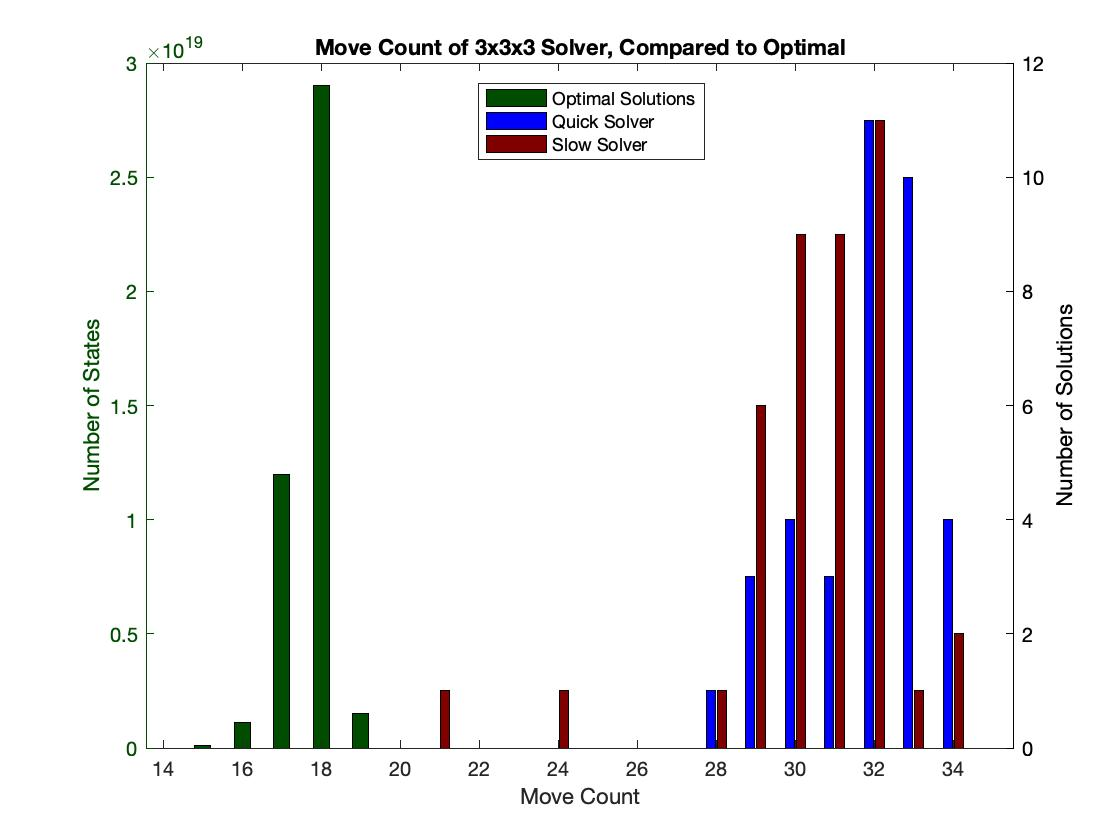
\includegraphics[width=5.5in]{movecount.jpg}
	\caption{We run the 3x3x3 solver for $42$ trials using two sets of parameters. The "quick" solver (blue) only looks for $2$ solutions from scrambled to a G1 state. For each possible solution, the solver then attempts to find solutions for the remainder of the puzzle (from G1 to solved), and returns the better of the two. The "slow" solver (red) instead finds $15$ possible solutions from G0 to G1 and tests each of the $15$, at the expense of running time. We can compare this distribution to the lengths of optimal solutions (green). For each of the $43$ quintillion states, there exists some optimal solution with length between $1$ move and $20$ moves; we plot number of states with each length, the vast majority of which fall between 16 and 19 moves \cite{god}. Due to the parameters set in later stages of the algorithm, the quick solver failed to find solutions for $6$ out of the $42$ scrambles, and the slow solver failed to solve $1$ scramble.}
	\label{fig:movecount}
\end{figure}

To test the implementation, we generate $42$ random scrambled states of the puzzle \cite{cstimer}. Then, for each scramble, we perform two runs of the solver: a slow run and a quick run. The slow run finds $15$ solutions to the first step (G0 to G1). The quick run only calculates $2$ possibilities instead of $15$, which results in faster runtime for both the G0 to G1 step and fewer computations for the remainder of the puzzle at the expense of slightly longer solutions.

The solver was run on a MacBook Pro with a 6-core 2.6 GHz processor and 16GB of RAM. Since the solver only takes advantage of a single core and uses less than $3$GB of RAM, five instances of the solver were run at any given time.

The quick solver took a median time of $9.05$ minutes (min: $2.78$ minutes, max: $140.5$ minutes). \fref{runtime} shows the runtime for each quick run. Unfortunately, the runtimes for the slow runs were lost; however, the slow runs took approximately $36$ hours in total.

\fref{movecount} compares the move counts for both the quick and slow runs. As expected, the slow solver, which performed additional computations, found slightly better solutions on average. The quick solver's solutions averaged $31.8$ moves (min: $28$, max: $34$), and the slow solver averaged $30.5$ moves (min: $21$, max: $34$). This figure also displays the distribution of the length of optimal solutions for all $43$ quintillion Rubik's Cube states \cite{god}. Out of all possible states, the vast majority are solved optimally in either $17$ or $18$ moves. Therefore, the solver in these $42$ trials found solutions that are approximately twice optimal in length.

We can compare these results to existing multi-phase algorithms. Kociemba's algorithm, which uses two phases instead of three, solves every puzzle in a maximum of $23$ moves and in a median of $18$ moves \cite{kociemba-dist}. Thistlethwaite's algorithm, which uses four phases, solves in an average of $31$ moves \cite{thistle-dist}. Though our solver uses three phases, there are many limitations (discussed below) that result in earlier phases (from G0 to G2) being suboptimal. For comparison, Kociemba's algorithm solves from G0 to G2 optimally in a single step. Our implementation always solves the last step from G2 to G3 optimally, like Kociemba's algorithm.

\begin{figure}
	\centering
    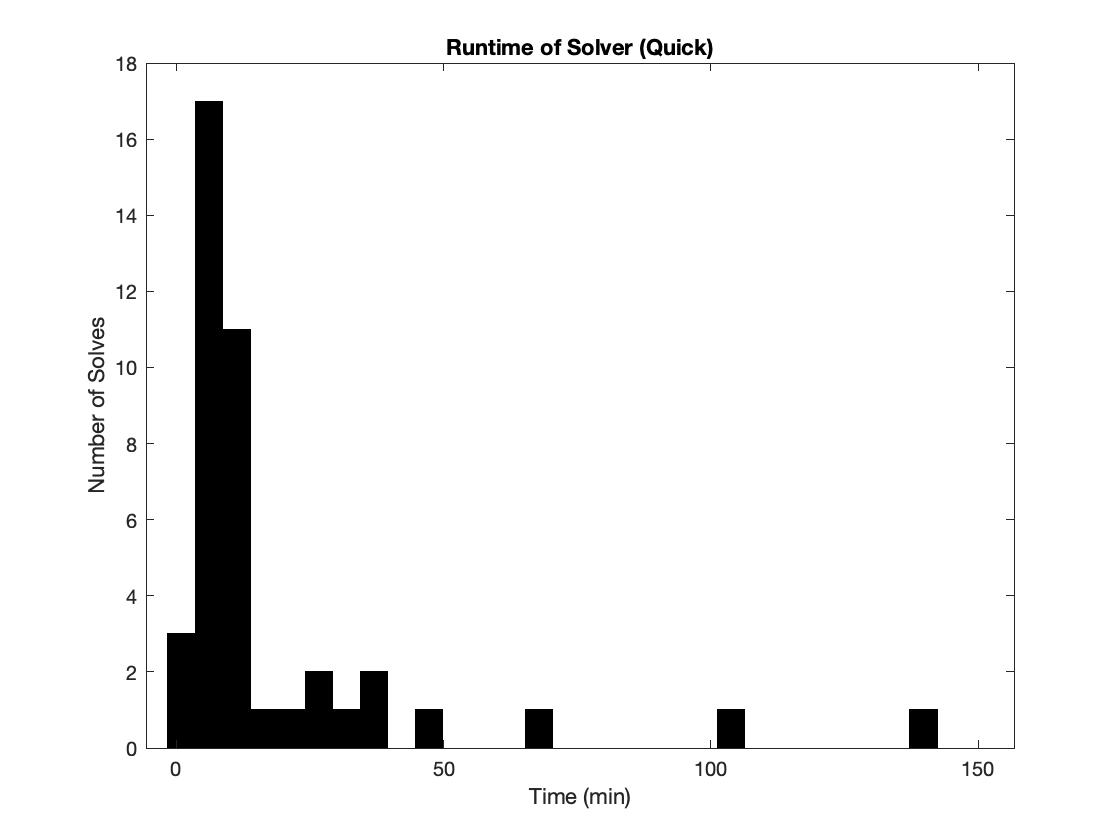
\includegraphics[width=5.5in]{runtime.jpg}
	\caption{Runtime of the "quick" solver for 42 trials. The quick solver only finds $2$ solutions from G0 (scrambled) to G1. A vast majority of scrambles were solved within $15$ minutes.}
	\label{fig:runtime}
\end{figure}

The numbers of $2$ and $15$ for quick and slow runs were chosen as proxies for determining how running longer affects solution length. It is possible to choose even higher numbers in order to find better solutions, at the expense of runtime. Similarly, we could also tweak parameters of other phases of the solver, which were kept fixed in these trials in a manner that balances runtime and solution length.

%========================================

\section{Limitations and Future Work}

There are a variety of limitations in our implementation that result in the algorithm being suboptimal, both in terms of runtime and in terms of the length of the solutions generated. % There are a variety of features in more established solvers, such as Cube Explorer, that are lacking here.

\subsection{Platform Limitations}
The solver is implemented using Python, and even simple operations like simulating the turning of a face require switching multiple entries within a NumPy array. Better-optimized solvers typically use lower-level languages, such as C or C++, and rely on specialized representations of the puzzle to perform these types of operations more efficiently \cite{kociemba-coord}.

\subsection{Symmetry Arguments}
The implementation above does not take into account the symmetry of different states of the puzzle. One example of this is that the algorithm arbitrarily chooses the face with the white center as the "up" face, and solves into the groups G1 and G2 relative to this choice. We could just as easily define any other face (say, the face with the red center) as the "up" face, which could lead to shorter solutions.

\subsection{Using Heuristics for Searching}
All brute-forced steps in this solver rely on a traditional breadth-first search. In contrast, recall that Korf's algorithm uses heuristics to prioritize performing certain moves that lead closer to a solved state.

We could apply a similar idea to this solver. This would involve replacing the breadth-first search currently used for brute-forcing with a heuristic-based depth-first search algorithm, such as Iterative Deepening A* \cite{ida}. This would also require generating lookup tables for the values of those heuristics, based on particular corner or edge properties.

\section{Conclusion}
In this project, we implemented a 3x3x3 Rubik's cube solver based on existing algorithms and techniques. The solver takes on the scale of minutes to generate solutions that are approximately twice optimal in length.

While this solver does not perform as well as other existing implementations, this implementation sheds light on many of the techniques that those solvers employ as they grapple with something that is inherently exponential in runtime.

\section{Bibliography}
\printbibliography[heading=none]


%========================================
\end{document}